\documentclass[11pt,handout]{beamer}
\usepackage[latin1]{inputenc}
\usepackage{amsmath}
\usepackage{framed}
\usepackage{listings}
% Graphics packages
\usepackage{graphicx}
\graphicspath{{figures/}}
\usepackage{pgf}
% Table packages
\usepackage{booktabs}
\usepackage{multirow}
\usepackage{tabularx}

\usetheme{Singapore}
\title[Changepoints in Open Source Evolution]{An Exploratory Study of Project Activity Changepoints in Open Source Software Evolution}
% \author[Walden]{James~Walden\\Center for Information Security\\Northern Kentucky University\\waldenj@nku.edu}
\author[]{James Walden \textsuperscript{1} \and Noah Burgin \inst{2} \and Kuljit Kaur\inst{3}}
\institute[]{\textsuperscript{1} Northern Kentucky University \and \inst{2} %
   University of Tennessee, Knoxville \and \inst{3} Guru Nanak Dev University} 
\date{}

% Setup logo with if statement to control placement
\newif\ifplacelogo % create a new conditional
\placelogotrue % set it to true
% Customize footline with NKU logo and no navigation symbols
% \logo{\ifplacelogo
%   \includegraphics[width=2cm, height=2cm, keepaspectratio]{nku-logo.jpg}~%
% \fi}

% Remove navigation circles for each slide below section names
\setbeamertemplate{navigation symbols}{}
\setbeamertemplate{mini frames}{}

% Add numbers in table of contents
\setbeamertemplate{section in toc}[sections numbered]

\begin{document}
\begin{frame}
    \titlepage
\end{frame}

\begin{frame}{Continuous Evolution or Punctuated Equilibrium?}
    Lehman's laws describe software evolution continuously
    \begin{itemize}
        \item IV - Average activity is invariant over program lifetime.
        \item VI - Functional content must be continually increased.
    \end{itemize}
    \vskip 5mm
    Lifecycle models describe evolution as punctuated by stages
    \begin{itemize}
        \item Waterfall model with different activity levels in each stage.
        \item Open source model is cyclical, looping over some stages.
    \end{itemize}
\end{frame}

\begin{frame}{Research Questions}
    Changepoints are when statistical properties of time series change.\\
    \vskip 3 mm
    Exploratory Research Questions:
    \begin{enumerate}
        \item How common are changepoints in open source project activity?
        \item What are the sizes and magnitudes of changes at changepoints?
    \end{enumerate}
    \vskip 3 mm
    Future Research Questions:
    \begin{enumerate}
        \item Can we identify changepoints that indicate project events?
        \item Can we identify patterns of changepoints that indicate lifecycle stages?
    \end{enumerate}
\end{frame}

\begin{frame}{Hackathon Project Goals}
    Identify changepoints in open source evolution time series
    \begin{itemize}
        \item Number of commits per month
        \item Number of unique authors per month
    \end{itemize}
    \vskip 3 mm
    Measure changepoints for practical significance
    \begin{itemize}
        \item Sign: positive or negative changes
        \item Magnitude: relative size of changes
    \end{itemize}
\end{frame}

\begin{frame}{Data Collection}
World of Code is an archive of 120+ million git repositories.\\
\vskip 5 mm
Selected projects that met the following criteria from WoC:
    \begin{itemize}
        \item At least 48 months between the first and last commit.
        \item At least 5000 commits.
        \item At least 50 authors.
    \end{itemize}
\vskip 3 mm
We found 8,919 projects that met these criteria.
\end{frame}

\begin{frame}{Data Collection using World of Code}
    Our data collection process consisted of the following steps:
    \begin{enumerate}
        \item Collect project metadata (name, age) from MongoDB.
        \item Select projects meeting our criteria for sufficient history.
        \item Use WoC maps to collect author and commit time series.
        \item Validate time series data (bad timestamps, missing data.)
        \item Identify changepoints with PELT-NP.
    \end{enumerate}
    \vskip 5mm
    Data and code are available at \url{https://github.com/woc-hack/inflection-points}
\end{frame}

\begin{frame}{Changes in Data Collection}
    \begin{itemize}
        \item Version S of the dataset provided information about root project as identified by Github.
        \item Creation of a new map reduced data collection time from days to hours.
        \item Writing a single file instead of one file per project reduced time from hours to minutes.
    \end{itemize}
\end{frame}

\begin{frame}{Changepoint Detection}
We evaluated three changepoint detection techniques:
    \begin{itemize}
        \item Segmented regression, which always finds a changepoint.
        \item Parametric changepoint detection algorithms like PELT.
        \item Nonparametric changepoint detection (NP-PELT).
    \end{itemize}
On two types of data:
    \begin{itemize}
        \item Synthetic time series constructed with known changepoints.
        \item Time series of monthly commits for OpenSSL, where we know changepoints exist.
    \end{itemize}
\end{frame}

\begin{frame}{OpenSSL Developer Activity}
    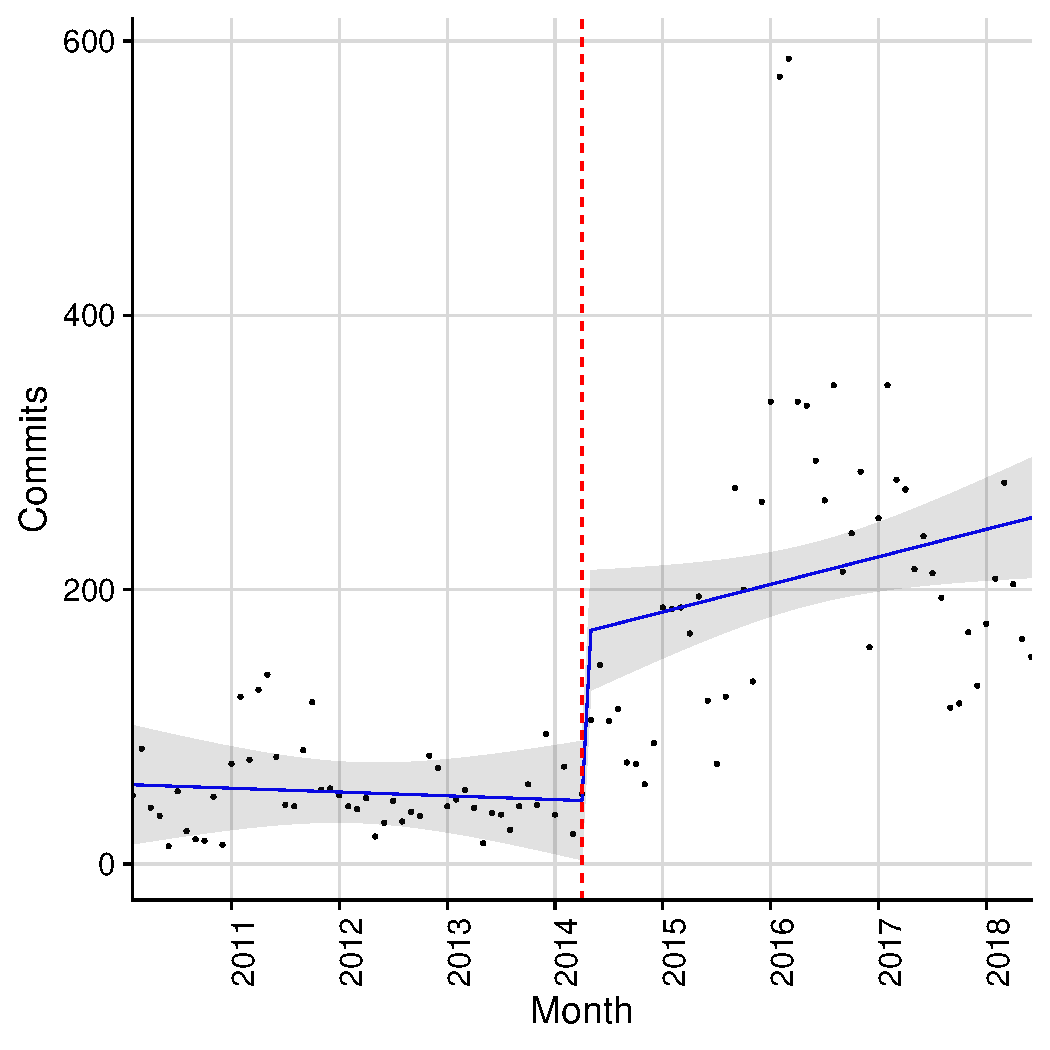
\includegraphics[width=0.5\textwidth,keepaspectratio]{ncommits.pdf}%
    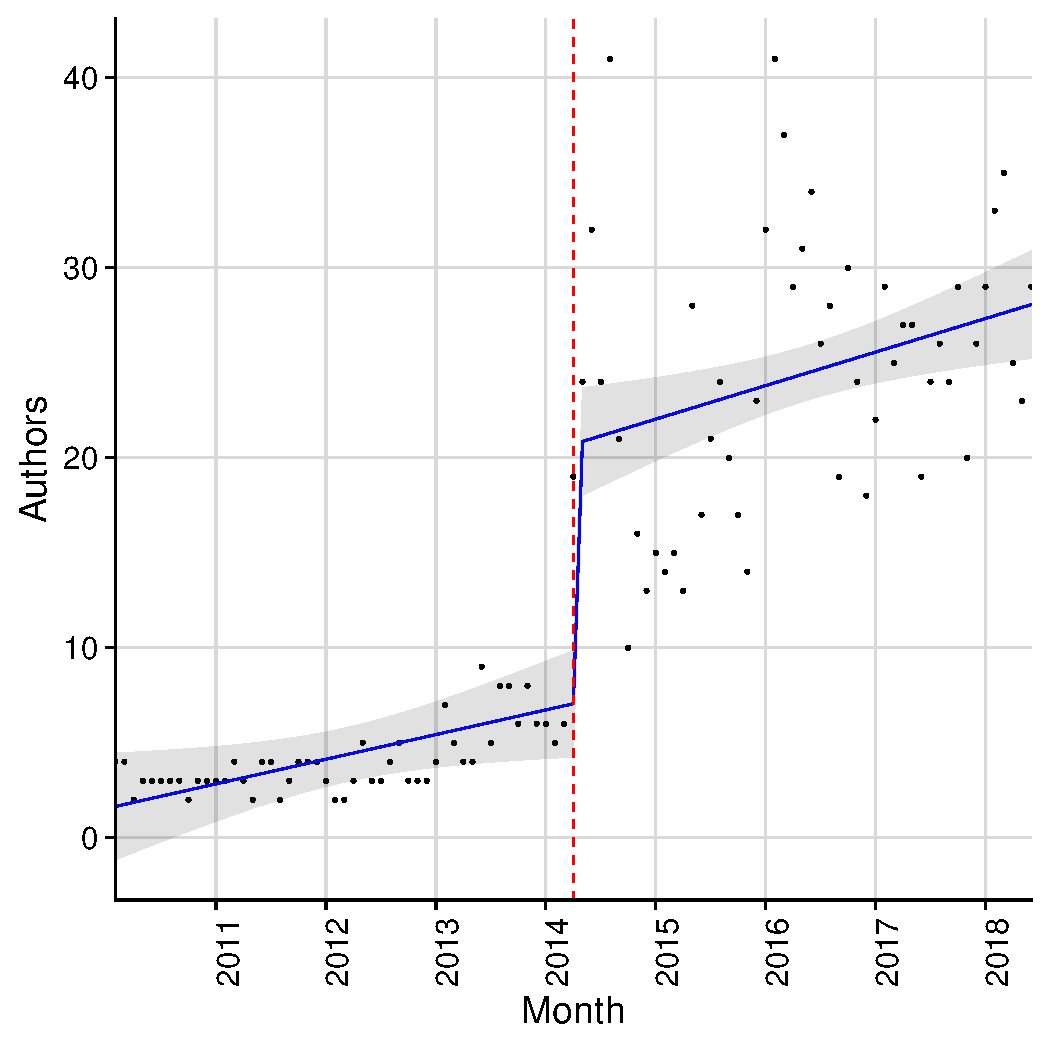
\includegraphics[width=0.5\textwidth,keepaspectratio]{nauthors.pdf}
\end{frame}

% The median number of changepoints in the commits per
% month time series was also three, with 32 projects having
% no changepoints. Most projects (90%) had between one and
% six changepoints. Outliers consisted of 27 projects with ten
% or more changepoints, including a single project with 16
% changepoints.
\begin{frame}{Projects by Number of Changepoints}
    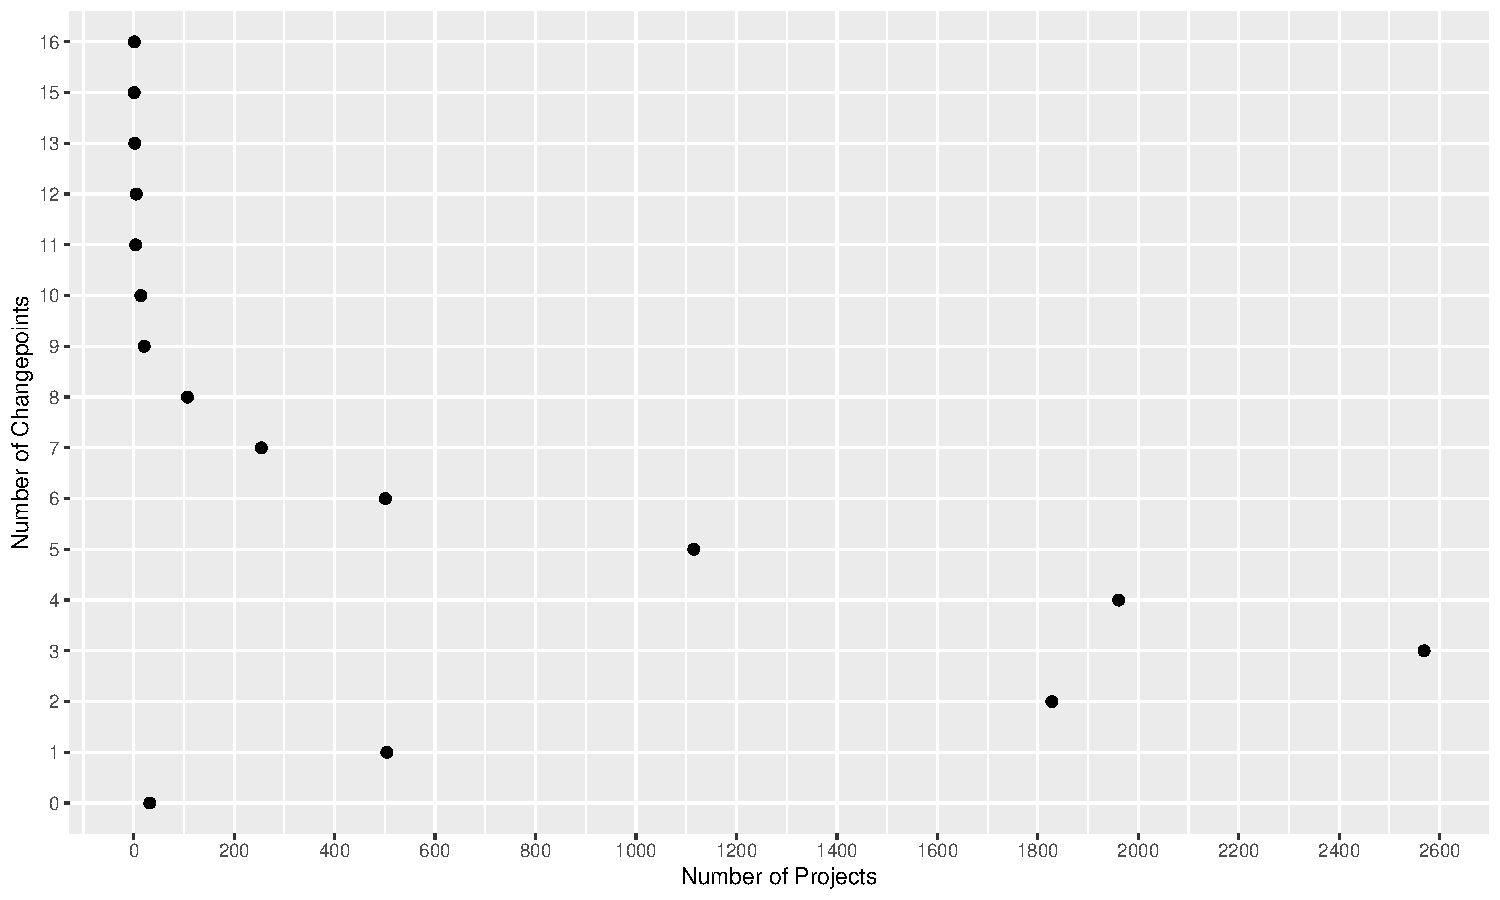
\includegraphics[width=\textwidth,keepaspectratio]{commit-changepoints.pdf}
\end{frame}

% We found a total of 31,416 changepoints in project commit
% time series, of which 15,342 (49%) were increases in commit
% activity and 16,047 (51%) were reductions in activity. We
% computed the magnitude of a changepoint as the difference in
% means in the number of monthly commits before and after the
% changepoint. The size of most changes were relatively small
% with the interquartile range (IQR) ranging between -75 to 87
% commits per month, but there was a substantial tail in both
% directions as can be seen in Figure 3.
\begin{frame}{Size of Changes in Commit Time Series}
    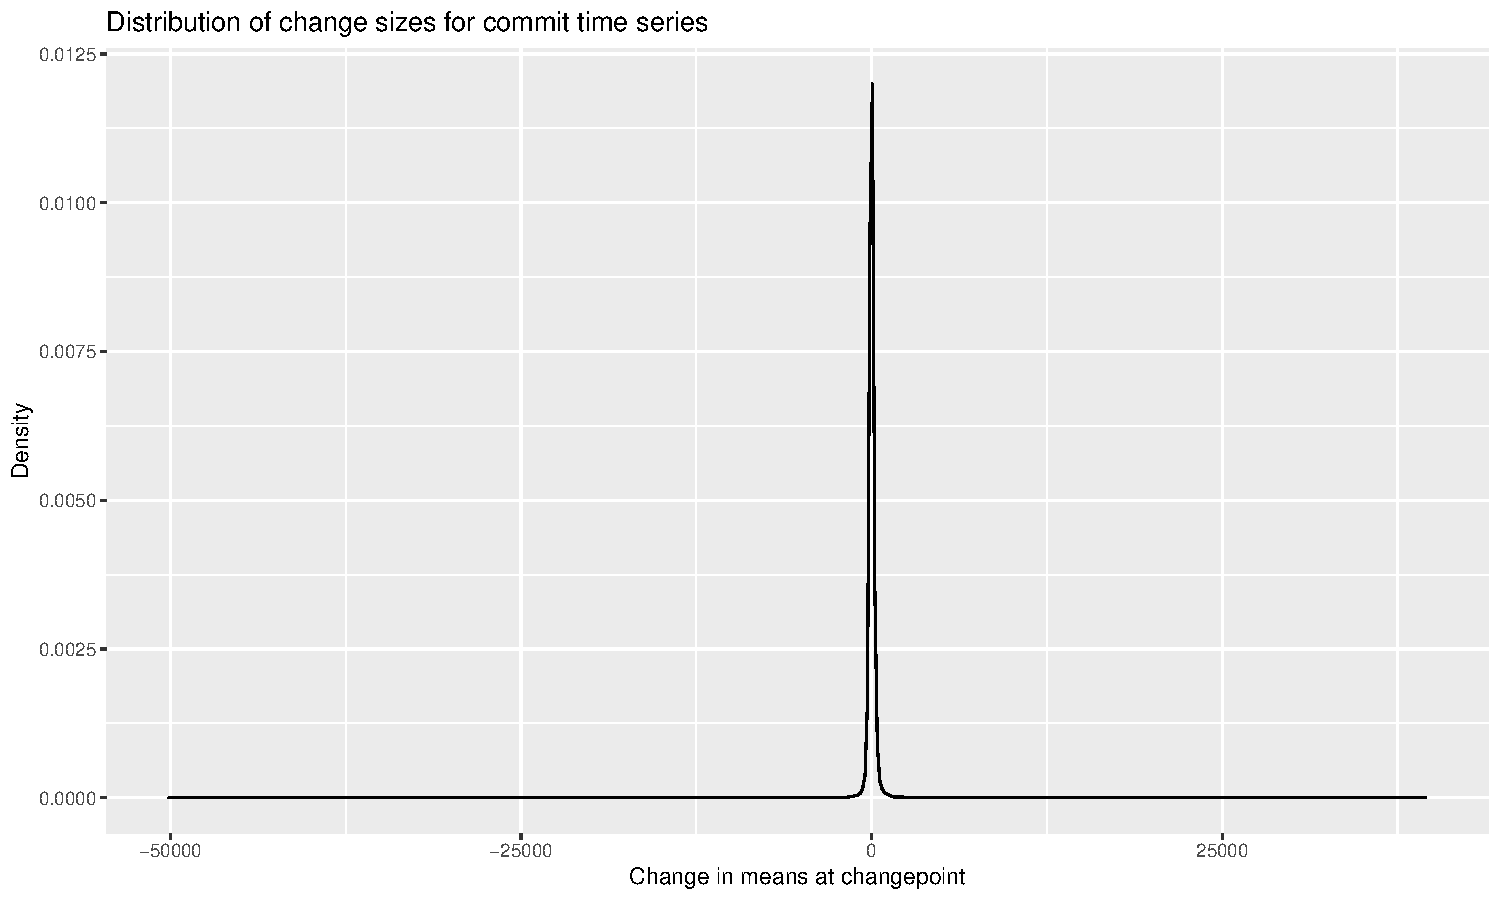
\includegraphics[width=\textwidth,keepaspectratio]{commit-changesizes.pdf}
\end{frame}

\begin{frame}{Conclusions and Future Work}
    Conclusions:
    \begin{itemize}
        \item Over 99\% of open source projects with extensive history have changepoints.
        \item Increases and decreases in project activity occur in roughly equal shares (51\% vs 49\%).
        \item Majority of changepoints range from -75 to 87 commits/month, but there are a number of huge outliers.
    \end{itemize}
    Future Work:
    \begin{itemize}
        \item Identify changepoint patterns, with a focus on large magnitude changes.
        \item Determine if there there are common lifecycle patterns identified by changepoints.
        \item Determine the impact of external events like COVID-19 on open source evolution.
    \end{itemize}
\end{frame}

% \begin{frame}[t]{Takeaways}
%     \fboxsep=0pt
%     \begin{minipage}[t]{0.58\linewidth}
%         \begin{itemize}
%             \item Security incidents combined with resources can dramatically improve an open source project.
%             \item Project activity and practices {\it may} be better indicators of security than vulnerability reports.
%             \item The OpenSSL dataset with code to produce the models, figures, and tables in the paper is available.
%         \end{itemize}
%     \end{minipage}%
%     \hfill%
%     \begin{minipage}[t]{0.4\linewidth}
%         \begin{framed}
%             {\bf Preprint:\\ \url{https://arxiv.org/abs/2005.14242}}
%         \end{framed}
%         \begin{framed}
%             {\bf Dataset:\\ \url{https://doi.org/10.6084/M9.FIGSHARE.11991348}}
%         \end{framed}
%     \end{minipage}
% \end{frame}

% \begin{frame}[t]{Takeaways}
%     \begin{itemize}
%         \item Security incidents combined with resources can dramatically improve an open source project.
%         \item Project activity and practices {\it may} be better indicators of security than vulnerability reports.
%         \item The OpenSSL dataset with code to produce the models, figures, and tables in the paper is available.
%     \end{itemize}
%     \begin{framed}
%         {\bf Preprint: \url{https://arxiv.org/abs/2005.14242}}
%     \end{framed}
%     \begin{framed}
%         {\bf Data: \url{https://doi.org/10.6084/M9.FIGSHARE.11991348}}
%     \end{framed}
% \end{frame}

% \begin{frame}[t]{Takeaways: Choosing Open Source Software}
%     \begin{itemize}
%         \item Past vulnerability history is not an indicator of security.
%             \begin{itemize}
%                 \item 66 (38\%) found in 16 years before Heartbleed.
%                 \item 105 (61\%) found in 5 years after Heartbleed.
%             \end{itemize}
%         \item Linus Law isn't true for all open source projects.
%             \begin{itemize}
%                 \item "Given enough eyeballs, all bugs are shallow."
%                 \item Low activity projects don't have "many eyeballs".
%                 \item Project activity may be a better indicator of security than vulnerability reports.
%             \end{itemize}
%     \end{itemize}
% \end{frame}

% \begin{frame}[t]{Takeaways: Developing Open Source Software}
%     \begin{itemize}
%         \item Low project activity may lead to technical debt.
%             \begin{itemize}
%                 \item High complexity, large amounts of old, unused code.
%                 \item Inconsistent style.
%             \end{itemize}
%         \item Projects can recover from major incidents if
%             \begin{itemize}
%                 \item Project activity increases, {\it and}
%                 \item Project activity directed towards technical debt.
%             \end{itemize}
%         \item Policies may be important in reducing technical debt.
%             \begin{itemize}
%                 \item Code contribution and style documents.
%                 \item Release planning with first end-of-life dates.
%                 \item Better contributions (consistent style, etc.)
%             \end{itemize}
%     \end{itemize}
% \end{frame}

\end{document}
